\chapter[SCP-014 混凝土人]{
    SCP-014 The Concrete Man\\
    SCP-014 混凝土人
}

\label{chap:SCP-014}

\begin{figure}[H]
    \centering
    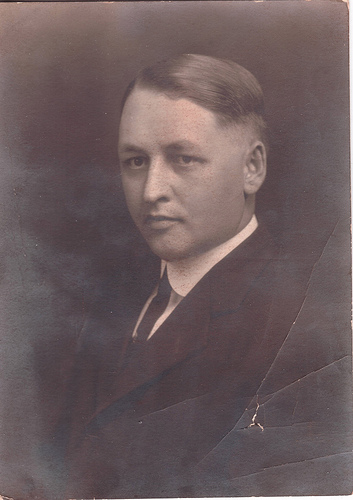
\includegraphics[width=0.5\linewidth]{images/SCP.014.jpg}
    \caption*{监禁前的SCP-014。}
\end{figure}

\bb{项目编号:}SCP-014

\bb{项目等级:}Safe

\bb{特殊收容措施:}SCP-014应安置在Site-██,可以坐在一把扶手椅中,最好面对窗户。应定期——最好是经常性地——提供音乐,而且曲目中不可包含创作于1937之后的作品。SCP-014的室中应安装保安摄像机。

\bb{描述:}SCP-014是一名白种人,男性,从外表看30岁左右,黑发棕眼,脸型稍圆。记录显示此人名叫\overtextnote{罗伯特·柴特福德(Robert Chetford)},1915年因妄想性精神病被幽禁在康涅狄格州的诺威奇精神病院。他声称自己被种下了永生不死的诅咒,身体也因此缓慢地变成混凝土。精神病院于1937年关闭,患者被转移到了五花八门的设施里。SCP-014引起基金会的注意是在19██年,传闻有位患者毫无衰老之兆,而且身体完全不能活动。经过进一步的调查,决定授权对其进行捕获。

外观上,SCP-014是一名普通男性,可他没有显现半点新陈代谢及衰老的迹象。他不饮食不排汗,断绝一切生命活动。他只在讲话时才些微换气,而且除了眼睛和发声器官,他彻头彻尾地硬如死尸。尽管几十年如一日地久居一处,他却皮肤不生褥疮,肌肉不见萎缩。他能够和人正常交谈,然而对遭到监禁后发生的事件却显得既漠不关心又缺乏足够的知识。

\bb{附录:}\\\ii{注:坦白说,如果采访这人时对他的背景一无所知,那我应该会觉得他是一个心智健全的个体,社会适应能力也不错,只不过得了瘫痪而已。照眼下的情况,我得下个结论:他是精神决定肉体这一理论的终极证明。他觉得自己是水泥,而且长生不老,那么他就会竭尽所能地实现这两个目标。甭管怎么着。█████博士}
